\begin{frame}[plain]
    \begin{center}
        \vspace{48pt}
        {\huge\bf センサーについて知ろう}
    \end{center}
\end{frame}

\begin{frame}
    \frametitle{ボタン}
    \begin{center}
        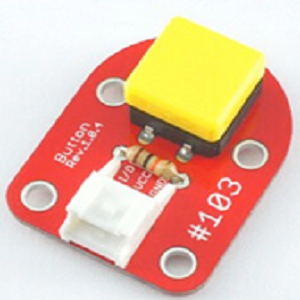
\includegraphics[width=0.4\textwidth]{images/chap05/text05-img028.png}
        \begin{itemize}
            \item ボタンが押されている間、値が1
            \item ボタンが押されていないと値が0
        \end{itemize}
    \end{center}
\end{frame}

\begin{frame}
    \frametitle{傾斜センサ}
    \begin{center}
        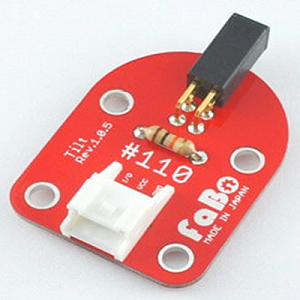
\includegraphics[width=0.4\textwidth]{images/chap05/text05-img018.png}
        \begin{itemize}
            \item 傾いているかどうかがわかる
            \item 黒い部分の中にたまが入っていて、かたむくと値が変わる
            \item 使用例:ストーブの安全装置
        \end{itemize}
    \end{center}
\end{frame}

\begin{frame}
    \frametitle{スイッチ}
    \begin{center}
        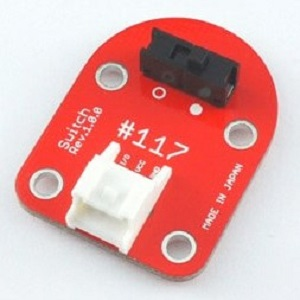
\includegraphics[width=0.4\textwidth]{images/chap05/text05-img019.jpg}
        \begin{itemize}
            \item スイッチがオンのとき値が1になる
            \item スイッチがオフのとき値が0になる
            \item オンのまま、オフのままにできる
        \end{itemize}
    \end{center}
\end{frame}

\begin{frame}
    \frametitle{リミットスイッチ}
    \begin{center}
        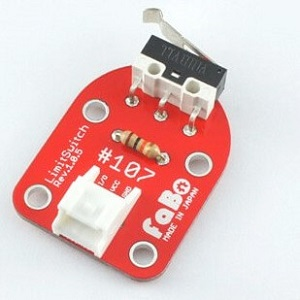
\includegraphics[width=0.4\textwidth]{images/chap05/text05-img020.jpg}
        \begin{itemize}
            \item スイッチが押されたとき値が1になる
            \item スイッチが押されていいないとき値が0になる
            \item 例:ふたがしまったかどうか
        \end{itemize}
    \end{center}
\end{frame}

\begin{frame}
    \frametitle{センサーをピンにつけてみよう}
    \begin{center}
        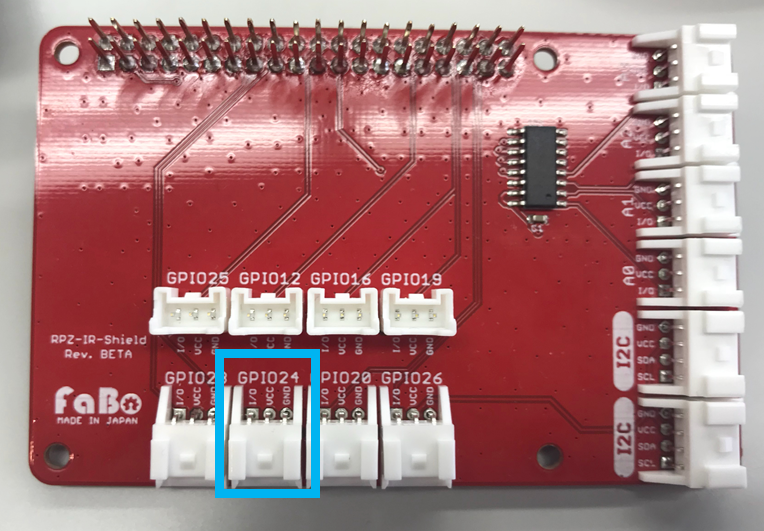
\includegraphics[width=0.7\textwidth]{images/chap05/text05-img029.png}
        \begin{itemize}
            \item GPIO23とLEDをつなげてみよう
            \item GPIO24と入力センサをつなげてみよう
            \item HSPでdigout.hspを動かしてみよう
        \end{itemize}
    \end{center}
\end{frame}

\begin{frame}[fragile]
    \frametitle{デジタル入力センサを使ったプログラム(digin.hsp)}
\begin{lstlisting}
#include "hsp3dish.as"
#include "rpz-gpio.as"

*main
	redraw 0
	pos 30,30
	mes "デジタル入力そうちでLEDを光らせよう"
	redraw 1
	if gpioin(24)=1 : goto *digital_on
	goto *digital_off
        
*digital_on
	gpio 23, 1
	wait 10
	goto *main

*digital_off
	gpio 23, 0
	wait 10
	goto *main 
\end{lstlisting}
\end{frame}

\begin{frame}[fragile]
    \frametitle{問題を解いてみよう}
    \begin{itemize}
        \item 教科書15ページ 問題5-5
        \begin{itemize}
            \item 5問を授業中にやる
        \end{itemize}
        \item 教科書15ページ 問題5-6
        \begin{itemize}
            \item 2問は宿題。時間があったら授業中にやる
        \end{itemize}

    \end{itemize}
\end{frame}